\documentclass[12pt,a4paper]{article}
\usepackage[utf8]{inputenc} % inutile avec XeLaTeX/LuaLaTeX
\usepackage[T1]{fontenc}
\usepackage{amsmath,amssymb,mathrsfs,tikz,times,pifont}
\usepackage{enumitem}
\usepackage{multicol}
\usepackage{lmodern}
\newcommand\circitem[1]{%
\tikz[baseline=(char.base)]{
\node[circle,draw=gray, fill=red!55,
minimum size=1.2em,inner sep=0] (char) {#1};}}
\newcommand\boxitem[1]{%
\tikz[baseline=(char.base)]{
\node[fill=cyan,
minimum size=1.2em,inner sep=0] (char) {#1};}}
\setlist[enumerate,1]{label=\protect\circitem{\arabic*}}
\setlist[enumerate,2]{label=\protect\boxitem{\alph*}}
\everymath{\displaystyle}
\usepackage[left=1cm,right=1cm,top=1cm,bottom=1.7cm]{geometry}
\usepackage[colorlinks=true, linkcolor=blue, urlcolor=blue, citecolor=blue]{hyperref}
\usepackage{array,multirow}
\usepackage[most]{tcolorbox}
\usepackage{varwidth}
\usepackage{float}
\tcbuselibrary{skins,hooks}
\usetikzlibrary{patterns}

\usepackage{pgfplots}
\pgfplotsset{compat=1.15}
\usepackage{mathrsfs}

\usepackage{amsmath}
\usepackage{amsfonts}
\usepackage{amssymb}
\usepackage{tkz-tab}
\usepackage{mdframed}
\usepackage{tikz}
\usetikzlibrary{arrows, shapes.geometric, fit}

\usepackage{xcolor}
\usepackage{tikz}
\usepackage{tkz-tab}
\usepackage{verbatim} % INDISPENSABLE pour l'environnement comment
\usepackage{yhmath}
\usepackage{array,multirow}
\usepackage[most]{tcolorbox}
\usepackage{varwidth}
\usepackage{graphicx}
\usetikzlibrary{shapes.geometric, positioning}
\usepackage{tabularx}
\usepackage{pifont} % Pour les symboles de coches et croix
\usepackage{eso-pic}         % Pour ajouter des éléments en arrière-plan
\usetikzlibrary{angles,quotes,arrows.meta}
% Définition du rouge pour les titres et soulignements
\definecolor{monRouge}{RGB}{180, 0, 0}

\usepackage{graphicx}
\usetikzlibrary{trees} % Nécessaire pour l'arbre
\usetikzlibrary{shapes.geometric, positioning}
\usepackage{tabularx}
\usepackage{pifont} % Pour les symboles de coches et croix
\usepackage{enumitem}
\usepackage{makecell}
% Définition des symboles du tableau
\newcommand{\coche}{{\color{red}\ding{51}}}
\newcommand{\croix}{{\color{red}\ding{55}}}

% Commande pour ajouter du texte en arrière-plan
\AddToShipoutPicture{
    \AtTextCenter{%
        \makebox[0pt]{\rotatebox{45}{\textcolor[gray]{0.6}{\fontsize{5cm}{5cm}\selectfont PGB}}}
    }
}

\begin{document}
% En-tête personnalisée
\begin{center}
    \Large\textbf{\underline{\textcolor{red}{Trigonométrie}}}\\[-0.1cm]
    \normalsize\textbf{Prof : M. BA} \hfill \textbf{Classe : 2ndS}\\[-0.1cm]
    \textbf{Année scolaire : 2025 -- 2026}
\end{center}

\begin{center}
    \fbox{
        \Large \textbf{Chapitre : Angles orientés et trigonométrie}
    }
\end{center}

\vspace{1.5em}

% --- SECTION I ---
\section*{%
    \color{monRouge}I - \underline{Angles orientés}%
}

% --- SUBSECTION 1 ---
\subsection*{%
    \color{monRouge} \underline{1 - Rappels et compléments}%
}

% --- SUBSUBSECTION a) ---
\subsubsection*{%
    \color{monRouge} \underline{a) Rappels : angles géométriques}%
}

% --- DÉFINITION ---
\noindent{\color{monRouge}\underline{Définition :}} 

Un angle géométrique est déterminé par deux demi-droites \textbf{[Ox)} et \textbf{[Oy)} de même origine \textbf{O}.

% --- SCHÉMA TIKZ ---
\begin{center}
    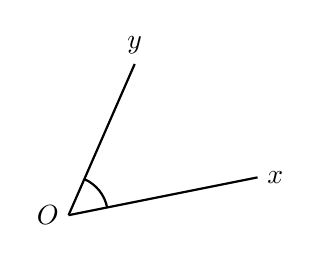
\begin{tikzpicture}[scale=1.2]
        % Points
        \coordinate (O) at (0,0);
        \coordinate (X) at (2,0.4); 
        \coordinate (Y) at (0.7,1.6); 

        % Dessin des demi-droites en noir
        \draw[thick] (O) -- (X);
        \draw[thick] (O) -- (Y);

        % Labels
        \node[left] at (O) {$O$};
        \node[right] at (X) {$x$};
        \node[above] at (Y) {$y$};

        % Arc de l'angle
        \pic [draw, angle radius=0.5cm, thick] {angle = X--O--Y};
    \end{tikzpicture}
\end{center}

\begin{comment}
\begin{center}
		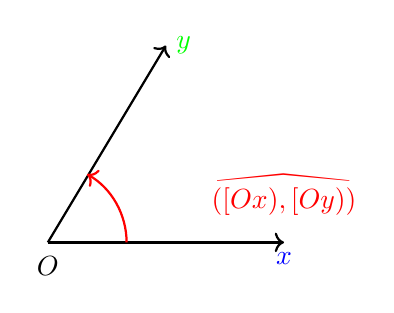
\begin{tikzpicture}
			\draw[->, thick] (0,0) -- (3,0) node[below] {\textcolor{blue}{$x$}};
			\draw[->, thick] (0,0) -- (1.5,2.5) node[right] {\textcolor{green}{$y$}};
			\node at (0,-0.3) {$O$};
			\draw[->, red, thick] (1,0) arc(0:60:1);
			\node at (3,0.6) {\textcolor{red}{$\widehat{\left( [Ox) , [ Oy)\right) }$}};
		\end{tikzpicture}
	\end{center}
\end{comment}

% --- ÉGALITÉ FINALE ---
\noindent Ici, on a : {\color{monRouge} $\widehat{xOy} = \widehat{yOx}$ }

% --- DÉFINITION : RADIAN ---
\noindent{\color{monRouge}\underline{Définition :}} \textbf{Radian}

\begin{itemize}
    \item[$*_{1}$] Un \textcolor{monRouge}{angle inscrit} dans un cercle est un angle dont le sommet appartient au cercle et ses côtés recoupent le cercle.
    
    \item[$*_{2}$] Un \textcolor{monRouge}{angle au centre} d'un cercle est un angle dont le sommet est le centre du cercle.
\end{itemize}

% --- SCHÉMA TIKZ ---
\begin{center}
    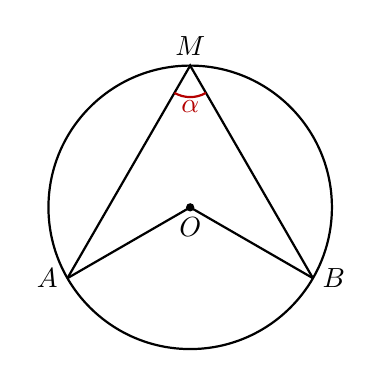
\begin{tikzpicture}[scale=1.5]
        % Le cercle
        \draw[thick] (0,0) circle (1.2cm);
        
        % Points de construction
        \coordinate (O) at (0,0);
        \coordinate (M) at (90:1.2);
        \coordinate (A) at (210:1.2);
        \coordinate (B) at (330:1.2);
        
        % Dessin de l'angle inscrit (MAB) en noir
        \draw[thick] (A) -- (M) -- (B);
        
        % Dessin de l'angle au centre (OAB) en noir
        \draw[thick] (A) -- (O) -- (B);
        
        % Labels des points
        \node[above] at (M) {$M$};
        \node[below] at (O) {$O$};
        \node[left] at (A) {$A$};
        \node[right] at (B) {$B$};
        
        % Petit arc rouge pour l'angle alpha
        \pic [draw, monRouge, thick, "$\alpha$", angle radius=0.4cm, angle eccentricity=1.3] {angle = A--M--B};
        
        % Point central (O) marqué
        \fill (O) circle (1pt);
    \end{tikzpicture}
\end{center}

\noindent \textcolor{monRouge}{$\widehat{AMB}$} est un angle inscrit \\
\noindent \textcolor{monRouge}{$\widehat{AOB}$} est un angle au centre

\begin{itemize}
    \item[$*_{3}$] L'angle \textcolor{monRouge}{$\alpha$} qui intercepte un arc de longueur égale au rayon du cercle est appelé \textcolor{monRouge}{radian}, noté \textcolor{monRouge}{rad}.
    
    \item[$*_{4}$] La longueur \textcolor{monRouge}{$l$} d'un arc de cercle de rayon $r$ intercepté par un angle au centre de mesure \textcolor{monRouge}{$\alpha$} en radian est égal à :
\end{itemize}

% --- SCHÉMA ET FORMULE ---
\begin{center}
    \begin{minipage}{0.4\textwidth}
        \centering
        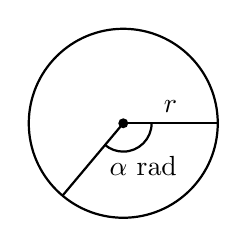
\begin{tikzpicture}[scale=1.2]
            % Le cercle
            \draw[thick] (0,0) circle (1cm);
            % Le centre O
            \fill (0,0) circle (1.5pt);
            % Rayons délimitant l'angle
            \draw[thick] (0,0) -- (0:1) node[midway, above] {$r$};
            \draw[thick] (0,0) -- (-130:1);
            % L'arc de l'angle alpha
            \draw[thick] (0.3,0) arc (0:-130:0.3);
            \node at (-65:0.5) {$\alpha$ rad};
        \end{tikzpicture}
    \end{minipage}
    \begin{minipage}{0.4\textwidth}
        \centering
        \color{monRouge}
        \setlength{\fboxrule}{1pt}
        \fbox{\Huge \rule[-0.4cm]{0pt}{1.2cm} $l = r\alpha$ }
    \end{minipage}
\end{center}

\begin{center}
    \textcolor{monRouge}{\underline{\Large Application}}
\end{center}

\noindent Calculer la longueur de l'arc de cercle de rayon $r$ intercepté par un angle au centre $\alpha$ rad avec $r = 2$ et $\alpha = \dfrac{\pi}{3}$

\begin{center}
    \textcolor{monRouge}{\underline{Correction}}
\end{center}

\noindent Soit $l$ la longueur de l'arc.

\noindent $l = r\alpha$ \\
$l = 2 \times \dfrac{\pi}{3}$ 

\vspace{0.5em}

\begin{center}
    \setlength{\fboxrule}{1pt}
    \fbox{\Large $l = \dfrac{2\pi}{3}$}
\end{center}

% --- REMARQUE ---
\noindent \textcolor{monRouge}{\underline{Remarque :}}

\begin{itemize}
    \item[i)] La mesure d'un angle géométrique appartient à l'intervalle $[0, \pi]$.
    \item[ii)] L'angle plat mesure \textcolor{monRouge}{$180^{\circ}$} (degré), \textcolor{monRouge}{$\pi$ rad} (radian) et \textcolor{monRouge}{$200$ gr} (grade).
\end{itemize}

\vspace{1em}

% --- APPLICATION ---
\begin{center}
    \textcolor{monRouge}{\underline{Application}}
\end{center}

\noindent Déterminer les mesures en radians, en grades de l'angle $\widehat{xOy}$ dans les cas suivants :

\begin{itemize}
    \item[a)] $mes(\widehat{xOy}) = 30^{\circ}$
    \item[b)] $mes(\widehat{xOy}) = 45^{\circ}$
    \item[c)] $mes(\widehat{xOy}) = 60^{\circ}$
    \item[d)] $mes(\widehat{xOy}) = 90^{\circ}$
\end{itemize}
\begin{center}
    \textcolor{monRouge}{\underline{Correction}}
\end{center}

Pour convertir les degrés ($D$) en radians ($R$) et en grades ($G$), on utilise la relation de proportionnalité :
\[ \frac{D}{180} = \frac{R}{\pi} = \frac{G}{200} \]

\begin{itemize}
    \item[a)] \textbf{Pour $30^{\circ}$ :}
    \begin{itemize}
        \item En radians : $R = \frac{30 \times \pi}{180} = \frac{\pi}{6}$ rad
        \item En grades : $G = \frac{30 \times 200}{180} = \frac{100}{3} \approx 33,33$ gr
    \end{itemize}

    \item[b)] \textbf{Pour $45^{\circ}$ :}
    \begin{itemize}
        \item En radians : $R = \frac{45 \times \pi}{180} = \frac{\pi}{4}$ rad
        \item En grades : $G = \frac{45 \times 200}{180} = 50$ gr
    \end{itemize}

    \item[c)] \textbf{Pour $60^{\circ}$ :}
    \begin{itemize}
        \item En radians : $R = \frac{60 \times \pi}{180} = \frac{\pi}{3}$ rad
        \item En grades : $G = \frac{60 \times 200}{180} = \frac{200}{3} \approx 66,66$ gr
    \end{itemize}

    \item[d)] \textbf{Pour $90^{\circ}$ :}
    \begin{itemize}
        \item En radians : $R = \frac{90 \times \pi}{180} = \frac{\pi}{2}$ rad
        \item En grades : $G = \frac{90 \times 200}{180} = 100$ gr
    \end{itemize}
\end{itemize}

\begin{center}
    \textcolor{monRouge}{\underline{\Large 2 - Propriétés}}
\end{center}

\begin{itemize}
    \item[i)] Deux angles inscrits qui interceptent le même arc ont des \textcolor{monRouge}{mesures égales}.
    
    \item[ii)] La mesure de l'angle au centre est le \textcolor{monRouge}{double} de la mesure de l'angle inscrit interceptant le même arc de cercle.
\end{itemize}

\begin{center}
    \textcolor{monRouge}{\underline{\Large Application}}
\end{center}

\noindent Soit $(\mathcal{C})$ un cercle de centre $O$ et de diamètre $[AB]$. \\
Montrer que pour tout point $M$ du cercle $(\mathcal{C})$ ($M \in \mathcal{C}$) distinct de $A$ et $B$, $AMB$ est un triangle rectangle en $M$.

% --- SCHÉMA TIKZ ---
\begin{center}
    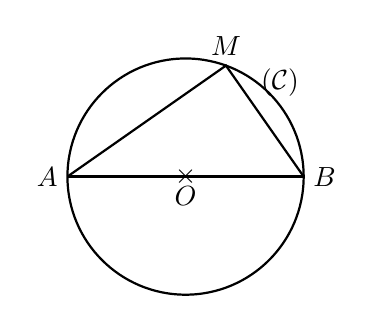
\begin{tikzpicture}[scale=1.5]
        % Le cercle
        \draw[thick] (0,0) circle (1cm);
        \node at (0.8,0.8) {$(\mathcal{C})$};
        
        % Diamètre [AB]
        \coordinate (O) at (0,0);
        \coordinate (A) at (-1,0);
        \coordinate (B) at (1,0);
        \draw[thick] (A) -- (B);
        \node[left] at (A) {$A$};
        \node[right] at (B) {$B$};
        \node[below] at (O) {$O$};
        \node at (0,0) {$\times$};
        
        % Point M et triangle
        \coordinate (M) at (70:1); % Point à 70 degrés sur le cercle
        \draw[thick] (A) -- (M) -- (B);
        \node[above] at (M) {$M$};
        
        % Symbole angle droit (optionnel mais pertinent pour la conclusion)
        %\draw (M) ++(-110:0.2) -- ++(-20:0.2) -- ++(70:0.2);
    \end{tikzpicture}
\end{center}

\begin{center}
    \textcolor{monRouge}{\underline{\Large Correction Rigoureuse}}
\end{center}

\paragraph{Données :} 
Soit $(\mathcal{C})$ un cercle de centre $O$. $[AB]$ est un diamètre de $(\mathcal{C})$, donc les points $A$, $O$ et $B$ sont alignés dans cet ordre. Le point $M$ appartient au cercle $(\mathcal{C})$ et est distinct de $A$ et $B$.

\paragraph{Démonstration :}
\begin{enumerate}
    \item L'angle $\widehat{AMB}$ est un \textbf{angle inscrit} dans le cercle $(\mathcal{C})$ qui intercepte l'arc de cercle $\overset{\frown}{AB}$.
    \item L'angle $\widehat{AOB}$ est l'\textbf{angle au centre} associé, car il intercepte le même arc $\overset{\frown}{AB}$.
    \item D'après la propriété de l'angle au centre, on sait que la mesure d'un angle inscrit est égale à la moitié de celle de l'angle au centre associé :
    \[ \widehat{AMB} = \frac{1}{2} \widehat{AOB} \]
    \item Or, $[AB]$ étant un diamètre passant par le centre $O$, l'angle $\widehat{AOB}$ est un \textbf{angle plat}. Sa mesure est donc :
    \[ \widehat{AOB} = 180^\circ \quad (\text{ou } \pi \text{ rad}) \]
    \item En substituant cette valeur dans la relation précédente, on obtient :
    \[ \widehat{AMB} = \frac{1}{2} \times 180^\circ = 90^\circ \]
\end{enumerate}

\paragraph{Conclusion :}
L'angle $\widehat{AMB}$ étant un angle droit ($90^\circ$), le triangle $AMB$ est \textbf{rectangle en $M$}.

\begin{center}
    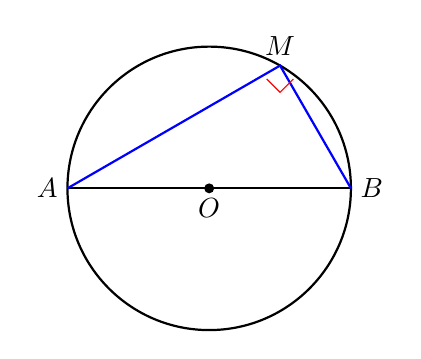
\begin{tikzpicture}[scale=1.2]
        \draw[thick] (0,0) circle (1.5);
        \coordinate (O) at (0,0);
        \coordinate (A) at (-1.5,0);
        \coordinate (B) at (1.5,0);
        \coordinate (M) at (60:1.5);
        
        \draw[thick] (A) -- (B);
        \draw[thick, blue] (A) -- (M) -- (B);
        
        \node[left] at (A) {$A$};
        \node[right] at (B) {$B$};
        \node[above] at (M) {$M$};
        \node[below] at (O) {$O$};
        \fill (O) circle (1.5pt);
        
        % Symbole de l'angle droit
        \begin{scope}[shift={(M)},rotate=-135]
            \draw[red] (0.2,0) -- (0.2,0.2) -- (0,0.2);
        \end{scope}
    \end{tikzpicture}
\end{center}

% --- SOUS-SECTION b) ---
\subsection*{%
    \color{monRouge}b - \underline{Compléments : quadrilatère inscriptible}%
}

\noindent Un quadrilatère est un polygone qui a 4 côtés.

\vspace{1em}

\noindent \textcolor{monRouge}{\underline{Remarque :}} On distingue 3 types de quadrilatère :

\begin{itemize}
    \item[*] \textbf{quadrilatère convexe :}
    
    \begin{minipage}{0.4\textwidth}
        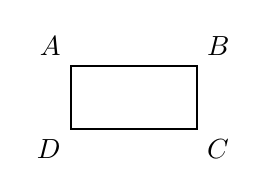
\begin{tikzpicture}[scale=0.8]
            \draw[thick] (0,0) node[below left]{$D$} -- (2,0) node[below right]{$C$} -- (2,1) node[above right]{$B$} -- (0,1) node[above left]{$A$} -- cycle;
        \end{tikzpicture}
    \end{minipage}
    \begin{minipage}{0.5\textwidth}
        $ABCD$ est un quadrilatère convexe.
    \end{minipage}
    
    \textit{Ex : carré, rectangle, trapèze...}

    \vspace{1em}

    \item[*] \textbf{quadrilatère concave :}
    
    \begin{minipage}{0.4\textwidth}
        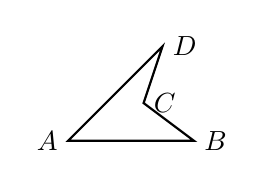
\begin{tikzpicture}[scale=0.8]
            \draw[thick] (0,0) node[left]{$A$} -- (2,0) node[right]{$B$} -- (1.2,0.6) node[right]{$C$} -- (1.5,1.5) node[right]{$D$} -- cycle;
        \end{tikzpicture}
    \end{minipage}
    \begin{minipage}{0.5\textwidth}
        $ABCD$ est un quadrilatère concave.
    \end{minipage}

    \vspace{1em}

    \item[*] \textbf{quadrilatère croisé :}
    
    \begin{minipage}{0.4\textwidth}
        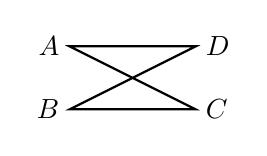
\begin{tikzpicture}[scale=0.8]
            \draw[thick] (0,1) node[left]{$A$} -- (2,0) node[right]{$C$} -- (0,0) node[left]{$B$} -- (2,1) node[right]{$D$} -- cycle;
        \end{tikzpicture}
    \end{minipage}
    \begin{minipage}{0.5\textwidth}
        $ABCD$ est un quadrilatère croisé.
    \end{minipage}
\end{itemize}

\noindent \textcolor{monRouge}{\underline{Définition 2 :}} \\
Un quadrilatère est dit \textcolor{monRouge}{inscriptible} dans un cercle lorsque ses 4 sommets sont sur le cercle.

\vspace{1em}

\noindent \textcolor{monRouge}{\underline{Ex :}}

\begin{center}
    % Premier exemple : Quadrilatère convexe
    \begin{minipage}{0.45\textwidth}
        \centering
        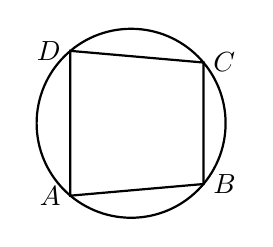
\begin{tikzpicture}[scale=1.2]
            \draw[thick] (0,0) circle (1cm);
            \coordinate (A) at (230:1);
            \coordinate (B) at (320:1);
            \coordinate (C) at (40:1);
            \coordinate (D) at (130:1);
            \draw[thick] (A) -- (B) -- (C) -- (D) -- cycle;
            \node[left] at (A) {$A$};
            \node[right] at (B) {$B$};
            \node[right] at (C) {$C$};
            \node[left] at (D) {$D$};
        \end{tikzpicture}
        \\[0.5em] $ABCD$ est inscriptible au cercle
    \end{minipage}
    \hfill
    % Deuxième exemple : Quadrilatère concave
    \begin{minipage}{0.45\textwidth}
        \centering
        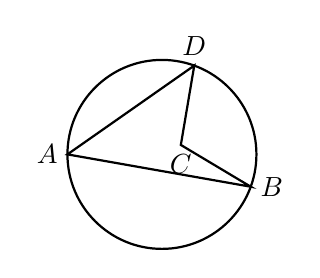
\begin{tikzpicture}[scale=1.2]
            \draw[thick] (0,0) circle (1cm);
            \coordinate (A) at (180:1);
            \coordinate (B) at (340:1);
            \coordinate (D) at (70:1);
            \coordinate (C) at (0.2,0.1); % Point intérieur pour la concavité
            \draw[thick] (A) -- (B) -- (C) -- (D) -- cycle;
            \node[left] at (A) {$A$};
            \node[right] at (B) {$B$};
            \node[below] at (C) {$C$};
            \node[above] at (D) {$D$};
        \end{tikzpicture}
        \\[0.5em] $ABCD$ est inscriptible au cercle
    \end{minipage}
\end{center}

\vspace{1.5em}

\noindent \textcolor{monRouge}{\underline{Propriété 1 :}} \\
Si un quadrilatère (non croisé) est inscrit dans un cercle, alors ses \textcolor{monRouge}{angles opposés sont supplémentaires}.

\begin{center}
    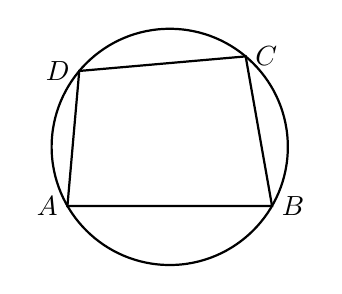
\begin{tikzpicture}[scale=1.5]
        \draw[thick] (0,0) circle (1cm);
        \coordinate (A) at (210:1);
        \coordinate (B) at (330:1);
        \coordinate (C) at (50:1);
        \coordinate (D) at (140:1);
        \draw[thick] (A) -- (B) -- (C) -- (D) -- cycle;
        \node[left] at (A) {$A$};
        \node[right] at (B) {$B$};
        \node[right] at (C) {$C$};
        \node[left] at (D) {$D$};
    \end{tikzpicture}
\end{center}

\noindent $\hat{A} + \hat{C} = 180^{\circ}$ \\
$\hat{B} + \hat{D} = 180^{\circ}$

% --- PROPRIÉTÉ 2 ---
\noindent \textcolor{monRouge}{\underline{Propriété 2 :}} \\
Si un quadrilatère convexe non croisé a ses angles opposés supplémentaires, alors il est \textcolor{monRouge}{inscriptible} dans un cercle.

\vspace{2em}

% --- APPLICATION ---
\begin{center}
    \textcolor{monRouge}{\underline{\Large Application}}
\end{center}

\noindent Soit $ABCD$ un quadrilatère tel que $\hat{B} = \hat{D} = 90^{\circ}$. \\
Montrer que $ABCD$ est inscriptible dans un cercle.

\vspace{1em}

% --- CORRECTION ---
\begin{center}
    \textcolor{monRouge}{\underline{Correction}}
\end{center}

\begin{center}
    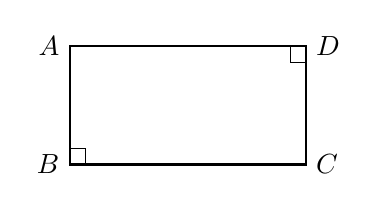
\begin{tikzpicture}
        % Dessin d'un rectangle simple pour l'illustration
        \draw[thick] (0,0) node[left]{$B$} -- (3,0) node[right]{$C$} -- (3,1.5) node[right]{$D$} -- (0,1.5) node[left]{$A$} -- cycle;
        % Symboles d'angles droits
        \draw (0,0.2) -- (0.2,0.2) -- (0.2,0);
        \draw (2.8,1.5) -- (2.8,1.3) -- (3,1.3);
    \end{tikzpicture}
\end{center}

\noindent On a : $\hat{B} = 90^{\circ}$ et $\hat{D} = 90^{\circ}$ \\
donc $\hat{B} + \hat{D} = 180^{\circ}$

\vspace{0.5em}

\noindent or $\hat{A} + \hat{B} + \hat{C} + \hat{D} = 360^{\circ}$ \\
$\hat{A} + 90^{\circ} + \hat{C} + 90^{\circ} = 360^{\circ}$ \\
$\hat{A} + \hat{C} = 360^{\circ} - 180^{\circ}$ \\
$\hat{A} + \hat{C} = 180^{\circ}$

\vspace{1em}

\noindent Les angles opposés sont supplémentaires, donc le quadrilatère $ABCD$ est bien inscriptible dans un cercle.

% --- SECTION 2 ---
\section*{%
    \color{monRouge} \underline{2 - Angles orientés}%
}

\subsection*{%
    \color{monRouge} \underline{a) Définition}%
}

\noindent Soient $[Ox)$ et $[Oy)$ deux demi-droites de même origine $O$. \\
On dit que ces demi-droites déterminent un \textbf{angle orienté} lorsqu'on choisit un sens de parcours du secteur angulaire et on note \textcolor{monRouge}{$(Ox, Oy)$}.

\begin{center}
    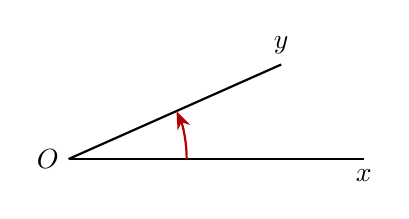
\begin{tikzpicture}[scale=1.5]
        % Axes
        \coordinate (O) at (0,0);
        \coordinate (X) at (2.5,0);
        \coordinate (Y) at (1.8,0.8);
        
        \draw[thick] (O) -- (X) node[below] {$x$};
        \draw[thick] (O) -- (Y) node[above] {$y$};
        \node[left] at (O) {$O$};
        
        % Flèche de sens de parcours en rouge
        \draw[->, >=Stealth, monRouge, thick] (1,0) arc (0:24:1);
    \end{tikzpicture}
\end{center}

\noindent \textcolor{monRouge}{$(\overrightarrow{Ox}, \overrightarrow{Oy}) = -(\overrightarrow{Oy}, \overrightarrow{Ox})$}

\subsection*{%
    \color{monRouge} \underline{b) Mesure principale}%
}

\noindent La \textcolor{monRouge}{mesure principale} d'un angle orienté est un réel $\alpha \in ]-\pi, \pi]$.

\vspace{1em}

\noindent \textcolor{monRouge}{\underline{Remarque :}} \\
Si $\alpha$ est mesure principale d'un angle alors : \\
\textcolor{monRouge}{$\theta = \alpha + 2k\pi$} avec $k \in \mathbb{Z}$, est aussi une mesure de l'angle.

\begin{center}
    \textcolor{monRouge}{\underline{\Large Application}}
\end{center}

\noindent Déterminer la mesure principale $\alpha$ de l'angle orienté $\theta$ dans les cas suivants :

\begin{itemize}
    \item[a)] $\theta = \dfrac{37}{3}\pi$
    \item[b)] $\theta = -\dfrac{71}{3}\pi$
    \item[c)] $\theta = \dfrac{119}{2}\pi$
\end{itemize}

\vspace{1.5em}

\noindent \textcolor{monRouge}{\underline{Correction}}

\noindent Pour déterminer la mesure principale $\alpha \in ]-\pi, \pi]$ d'un angle $\theta$, on cherche l'entier $k$ tel que :
\[ \alpha = \theta - 2k\pi \]

\begin{itemize}
    \item[a)] \textbf{Pour $\theta = \dfrac{37}{3}\pi$}
    
    $\dfrac{37}{3} \approx 12,33$. L'entier pair le plus proche est $12$.
    \[ \alpha = \dfrac{37\pi}{3} - 12\pi = \dfrac{37\pi - 36\pi}{3} = \dfrac{\pi}{3} \]
    $\dfrac{\pi}{3} \in ]-\pi, \pi]$, donc \textcolor{monRouge}{$\alpha = \dfrac{\pi}{3}$}.

    \item[b)] \textbf{Pour $\theta = -\dfrac{71}{3}\pi$}
    
    $-\dfrac{71}{3} \approx -23,66$. L'entier pair le plus proche est $-24$.
    \[ \alpha = -\dfrac{71\pi}{3} - (-24\pi) = -\dfrac{71\pi}{3} + \dfrac{72\pi}{3} = \dfrac{\pi}{3} \]
    $\dfrac{\pi}{3} \in ]-\pi, \pi]$, donc \textcolor{monRouge}{$\alpha = \dfrac{\pi}{3}$}.

    \item[c)] \textbf{Pour $\theta = \dfrac{119}{2}\pi$}
    
    $\dfrac{119}{2} = 59,5$. L'entier pair le plus proche est $60$.
    \[ \alpha = \dfrac{119\pi}{2} - 60\pi = \dfrac{119\pi - 120\pi}{2} = -\dfrac{\pi}{2} \]
    $-\dfrac{\pi}{2} \in ]-\pi, \pi]$, donc \textcolor{monRouge}{$\alpha = -\dfrac{\pi}{2}$}.
\end{itemize}

\begin{center}
    \textcolor{monRouge}{\underline{\Large Exercice de Synthèse}}
\end{center}

\noindent \textbf{Partie A : Géométrie Plane} \\
Soit $(\mathcal{C})$ un cercle de centre $O$. Soit $[AB]$ un diamètre de ce cercle. On considère un point $C$ sur le cercle tel que $\widehat{BOC} = 60^\circ$.
\begin{enumerate}
    \item Quelle est la nature du triangle $ABC$ ? Justifier.
    \item Calculer la mesure de l'angle inscrit $\widehat{BAC}$.
    \item Soit $D$ le point diamétralement opposé à $C$. Démontrer que le quadrilatère $ACBD$ est un rectangle. Est-il inscriptible ?
\end{enumerate}

\noindent \textbf{Partie B : Angles orientés} \\
On considère l'angle orienté $\theta = (\overrightarrow{OA}, \overrightarrow{OC})$.
\begin{enumerate}
    \item Donner une mesure de $\theta$ en degrés, puis en radians.
    \item Déterminer la mesure principale de l'angle $\phi = \dfrac{25\pi}{3}$.
\end{enumerate}

\vspace{1.5em}

\begin{center}
    \textcolor{monRouge}{\underline{\Large Correction}}
\end{center}

\noindent \textbf{Partie A}
\begin{enumerate}
    \item $C$ appartient au cercle de diamètre $[AB]$. Tout triangle inscrit dans un cercle ayant pour côté un diamètre est rectangle. Donc \textbf{$ABC$ est rectangle en $C$}.
    \item $\widehat{BAC}$ est un angle inscrit qui intercepte l'arc $\wideparen{BC}$. $\widehat{BOC}$ est l'angle au centre associé.
    \[ \widehat{BAC} = \frac{1}{2} \widehat{BOC} = \frac{1}{2} (60^\circ) = \mathbf{30^\circ} \]
    \item Les diagonales $[AB]$ et $[CD]$ sont des diamètres du cercle. Elles ont donc la même longueur et se coupent en leur milieu $O$. Un quadrilatère dont les diagonales sont égales et se coupent en leur milieu est un \textbf{rectangle}.
    Tout rectangle est \textbf{inscriptible} car ses angles opposés sont supplémentaires ($90^\circ + 90^\circ = 180^\circ$).
\end{enumerate}

\noindent \textbf{Partie B}
\begin{enumerate}
    \item Comme $A, O, B$ sont alignés, $\widehat{AOC} = 180^\circ - \widehat{BOC} = 180 - 60 = \mathbf{120^\circ}$.
    En radians : $R = \dfrac{120 \times \pi}{180} = \mathbf{\dfrac{2\pi}{3} \text{ rad}}$.
    \item Pour $\phi = \dfrac{25\pi}{3}$ :
    $\dfrac{25}{3} \approx 8,33$. L'entier pair le plus proche est $8$.
    \[ \alpha = \frac{25\pi}{3} - 8\pi = \frac{25\pi - 24\pi}{3} = \mathbf{\dfrac{\pi}{3}} \]
    La mesure principale est $\dfrac{\pi}{3}$ car elle appartient à $]-\pi, \pi]$.
\end{enumerate}

\begin{center}
    \textcolor{monRouge}{\underline{\Large Exercice : Mesures Principales}}
\end{center}

\noindent Déterminer la mesure principale $\alpha \in ]-\pi ; \pi]$ des angles orientés suivants :

\begin{enumerate}
    \item[a)] $\theta_1 = \dfrac{47\pi}{4}$
    \item[b)] $\theta_2 = -\dfrac{31\pi}{6}$
    \item[c)] $\theta_3 = \dfrac{2026\pi}{3}$
    \item[d)] $\theta_4 = -\dfrac{15\pi}{2}$
    \item[e)] $\theta_5 = -15\pi$
    \item[f)] $\theta_6 = 40\pi$
\end{enumerate}

\vspace{2em}

\begin{center}
    \textcolor{monRouge}{\underline{\Large Correction détaillée}}
\end{center}

\begin{itemize}
    \item[a)] \textbf{Pour $\theta_1 = \dfrac{47\pi}{4}$} :
    \\ $\dfrac{47}{4} = 11,75$. L'entier pair le plus proche est $12$.
    \\ $\alpha = \dfrac{47\pi}{4} - 12\pi = \dfrac{47\pi - 48\pi}{4} = \mathbf{-\dfrac{\pi}{4}}$
    \\ $-\dfrac{\pi}{4} \in ]-\pi ; \pi]$, c'est la mesure principale.

    \vspace{1em}

    \item[b)] \textbf{Pour $\theta_2 = -\dfrac{31\pi}{6}$} :
    \\ $-\dfrac{31}{6} \approx -5,16$. L'entier pair le plus proche est $-6$ (car $-4$ donnerait un résultat hors intervalle).
    \\ $\alpha = -\dfrac{31\pi}{6} - (-6\pi) = -\dfrac{31\pi}{6} + \dfrac{36\pi}{6} = \mathbf{\dfrac{5\pi}{6}}$
    \\ $\dfrac{5\pi}{6} \in ]-\pi ; \pi]$, c'est la mesure principale.

    \vspace{1em}

    \item[c)] \textbf{Pour $\theta_3 = \dfrac{2026\pi}{3}$} :
    \\ $\dfrac{2026}{3} \approx 675,33$. L'entier pair le plus proche est $676$.
    \\ $\alpha = \dfrac{2026\pi}{3} - 676\pi = \dfrac{2026\pi - 2028\pi}{3} = \mathbf{-\dfrac{2\pi}{3}}$
    \\ $-\dfrac{2\pi}{3} \in ]-\pi ; \pi]$, c'est la mesure principale.

    \vspace{1em}

    \item[d)] \textbf{Pour $\theta_4 = -\dfrac{15\pi}{2}$} :
    \\ $-\dfrac{15}{2} = -7,5$. L'entier pair le plus proche est $-8$.
    \\ $\alpha = -\dfrac{15\pi}{2} - (-8\pi) = -\dfrac{15\pi}{2} + \dfrac{16\pi}{2} = \mathbf{\dfrac{\pi}{2}}$
    \\ $\dfrac{\pi}{2} \in ]-\pi ; \pi]$, c'est la mesure principale.
    \item[e)] \textbf{Pour $\theta_5 = -15\pi$} :
    \\ $-15$ est un nombre impair. On peut écrire $-15\pi = -14\pi - \pi$ ou $-16\pi + \pi$.
    \\ Pour être dans l'intervalle $]-\pi ; \pi]$, on choisit l'entier pair le plus proche qui permet de rester dans la borne.
    \\ $-15\pi - (-16\pi) = \pi$.
    \\ $\pi \in ]-\pi ; \pi]$, donc la mesure principale est \textbf{$\pi$}.
    
    \vspace{1em}

    \item[f)] \textbf{Pour $\theta_6 = 40\pi$} :
    \\ $40$ est déjà un nombre pair. Cela signifie que l'angle correspond à 20 tours complets du cercle.
    \\ $\alpha = 40\pi - 40\pi = 0$.
    \\ $0 \in ]-\pi ; \pi]$, donc la mesure principale est \textbf{$0$}.
\end{itemize}

% --- SECTION C (IMAGE 2) ---

\subsection*{%
    \color{monRouge} \underline{C) Propriétés des angles orientés}%
}
Soient $\vec{u}$, $\vec{v}$ et $\vec{w}$ 3 vecteurs non nuls.

\vspace{1em}

\noindent $P_1 : (\vec{u}, \vec{u}) = 0$ \\
$P_2 : (\vec{u}, \vec{v}) = -(\vec{v}, \vec{u})$ \\
$P_3 : (k\vec{u}, k'\vec{v}) = \begin{cases} (\vec{u}, \vec{v}) & \text{si } kk' > 0 \\ \pi + (\vec{u}, \vec{v}) & \text{si } kk' < 0 \end{cases}$

\vspace{1em}

\noindent \textcolor{monRouge}{$P_4 :$ \underline{Relation de Chasles}} \\
$(\vec{u}, \vec{v}) = (\vec{u}, \vec{w}) + (\vec{w}, \vec{v})$

\begin{center}
    \textcolor{monRouge}{\underline{\Large Application}}
\end{center}

\noindent Sachant que $(\vec{u}, \vec{v}) = \dfrac{\pi}{3}$ et $(\vec{w}, \vec{v}) = -\dfrac{\pi}{4}$, déterminer :

\begin{itemize}
    \item[a)] $(\vec{u}, 2\vec{v})$
    \item[b)] $(-3\vec{u}, \vec{v})$
    \item[c)] $(\vec{u}, \vec{w})$
    \item[d)] $(-2\vec{v}, 5\vec{u})$
    \item[e)] $(\vec{u}, -\vec{u})$
\end{itemize}

    \subsection*{%
    \color{monRouge} \underline{II - Trigonométrie}%
}


\noindent \textbf{\textcolor{monRouge}{\underline{1 - Cosinus, sinus et tangente}}}

\subsection*{%
    \color{monRouge} \underline{a) Définitions}%
}

\noindent \textcolor{monRouge}{\underline{Définition 1 :}} \\
Dans un repère orthonormé $(O, \vec{i}, \vec{j})$, on appelle \textcolor{monRouge}{cercle trigonométrique}, le cercle de centre $O$ et de rayon $1$ orienté dans le \textcolor{monRouge}{sens direct} (sens contraire des aiguilles d'une montre). Le sens direct est aussi appelé sens trigonométrique.

\begin{center}
    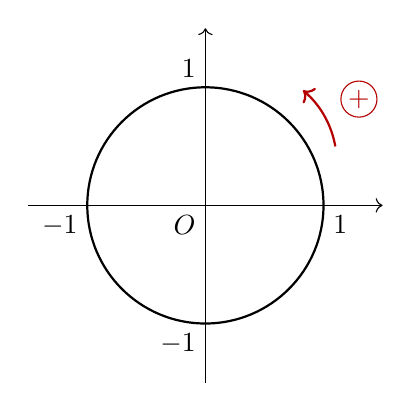
\begin{tikzpicture}[scale=1.5]
        % Axes
        \draw[->] (-1.5,0) -- (1.5,0);
        \draw[->] (0,-1.5) -- (0,1.5);
        
        % Cercle
        \draw[thick] (0,0) circle (1cm);
        
        % Origine et unités
        \node[below left] at (0,0) {$O$};
        \node[below right] at (1,0) {$1$};
        \node[below left] at (-1,0) {$-1$};
        \node[above left] at (0,1) {$1$};
        \node[below left] at (0,-1) {$-1$};
        
        % Symbole sens direct (plus dans un cercle)
        \draw[->, monRouge, thick] (1.1,0.5) arc (10:50:0.8);
        \node[monRouge, draw, circle, inner sep=1pt] at (1.3,0.9) {$+$};
    \end{tikzpicture}
\end{center}

\noindent \textcolor{monRouge}{\underline{Définition :}} \\
On munit le plan d'un cercle trigonométrique $(\mathcal{C})$ dans un repère $(O, \vec{i}, \vec{j})$. \\
Soient $M \in (\mathcal{C})$ et $\alpha \in ]-\pi, \pi]$ tel que $\alpha = (\vec{i}, \overrightarrow{OM})$.

\begin{center}
    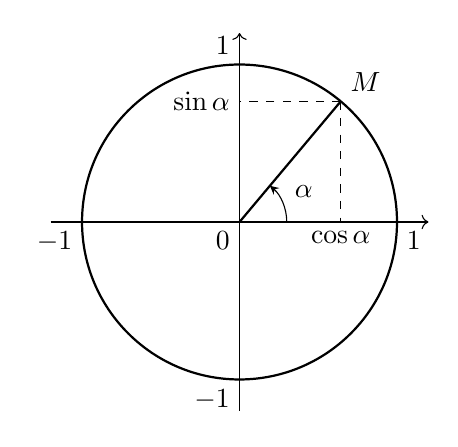
\begin{tikzpicture}[scale=2]
        % Axes
        \draw[->] (-1.2,0) -- (1.2,0);
        \draw[->] (0,-1.2) -- (0,1.2);
        
        % Cercle
        \draw[thick] (0,0) circle (1cm);
        
        % Point M et angle
        \coordinate (M) at (50:1);
        \draw[thick] (0,0) -- (M);
        \node[above right] at (M) {$M$};
        \draw[->, >=stealth] (0.3,0) arc (0:50:0.3);
        \node at (25:0.45) {$\alpha$};
        
        % Projections (pointillés)
        \draw[dashed] (M) -- ({cos(50)},0) node[below] {$\cos \alpha$};
        \draw[dashed] (M) -- (0,{sin(50)}) node[left] {$\sin \alpha$};
        
        % Unités et Origine
        \node[below left] at (0,0) {$0$};
        \node[below right] at (1,0) {$1$};
        \node[below left] at (-1,0) {$-1$};
        \node[above left] at (0,1) {$1$};
        \node[below left] at (0,-1) {$-1$};
    \end{tikzpicture}
\end{center}

\begin{itemize}
    \item L'\textcolor{monRouge}{abscisse} du point $M$ dans $(O, \vec{i}, \vec{j})$ est appelée \textcolor{monRouge}{cosinus} de $\alpha$ et est notée \textcolor{monRouge}{$\cos \alpha$}.
    \item L'\textcolor{monRouge}{ordonnée} du point $M$ dans $(O, \vec{i}, \vec{j})$ est appelée \textcolor{monRouge}{sinus} de $\alpha$ et est notée \textcolor{monRouge}{$\sin \alpha$}.
\end{itemize}

\noindent \textcolor{monRouge}{\underline{Remarque :}} \\
Soit $\alpha \in ]-\pi, \pi]$. On appelle \textcolor{monRouge}{tangente} de $\alpha$ notée $\tan \alpha$ le réel défini par :
\begin{center}
    \color{monRouge} \fbox{$\tan \alpha = \dfrac{\sin \alpha}{\cos \alpha}$}
\end{center}

\noindent $\tan \alpha$ existe ssi $\alpha \neq \dfrac{\pi}{2} + k\pi, k \in \mathbb{Z}$.

\vspace{1.5em}

\subsection*{%
    \color{monRouge} \underline{b) Propriétés : conséquences de la définition}%
}
\vspace{1em}

\noindent \textcolor{monRouge}{\underline{Propriété 1 :}} Pour tout réel $\alpha$, on a :
\begin{itemize}
    \item[i)] $\cos(\alpha + 2k\pi) = \cos \alpha, \quad k \in \mathbb{Z}$
    \item[ii)] $\sin(\alpha + 2k\pi) = \sin \alpha, \quad k \in \mathbb{Z}$
\end{itemize}

\noindent \textcolor{monRouge}{\underline{Propriété 2 :}} Pour tout réel $\alpha$, on a :
\begin{itemize}
    \item[i)] $-1 \le \cos \alpha \le 1$
    \item[ii)] $-1 \le \sin \alpha \le 1$
\end{itemize}

\vspace{1.5em}

\noindent \textcolor{monRouge}{\underline{Propriété 3 :}} Pour tout réel $\alpha$, on a :
\begin{center}
    $\cos^2(\alpha) + \sin^2(\alpha) = 1$
\end{center}


\noindent \textcolor{monRouge}{\underline{Preuve :}}

\begin{center}
    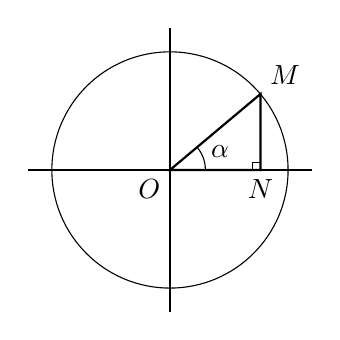
\begin{tikzpicture}[scale=1.5]
        % Axes
        \draw (0,-1.2) -- (0,1.2);
        \draw (-1.2,0) -- (1.2,0);
        
        % Cercle
        \draw (0,0) circle (1cm);
        
        % Triangle OMN
        \coordinate (O) at (0,0);
        \coordinate (M) at (40:1);
        \coordinate (N) at ({cos(40)},0);
        
        \draw[thick] (O) -- (M) -- (N) -- cycle;
        
        % Labels
        \node[below left] at (O) {$O$};
        \node[above right] at (M) {$M$};
        \node[below] at (N) {$N$};
        
        % Angle alpha
        \draw (0.3,0) arc (0:40:0.3);
        \node at (20:0.45) {$\alpha$};
        
        % Angle droit
        \draw (0.7,0) -- (0.7,0.06) -- ({cos(40)},0.06);
    \end{tikzpicture}
\end{center}

\noindent Soit le triangle $OMN$ rectangle en $N$, d'après le théorème de Pythagore, on a :
\[ ON^2 + MN^2 = OM^2 \]

\noindent $\begin{cases} ON = \cos \alpha \\ MN = \sin \alpha \\ OM = 1 \end{cases}$

\vspace{1em}

\noindent Donc $\cos^2 \alpha + \sin^2 \alpha = 1$

\noindent \textcolor{monRouge}{\underline{Exercice :}} \\
Soit $\alpha \neq \dfrac{\pi}{2} + k\pi, \quad k \in \mathbb{Z}$

\vspace{0.5em}

\noindent Montrer que $1 + \tan^2 \alpha = \dfrac{1}{\cos^2 \alpha}$

\vspace{1.5em}

\subsection*{%
    \color{monRouge} \underline{c) Étude du signe du cosinus et du sinus dans les 4 quadrants}%
}
\vspace{1em}

\begin{center}
    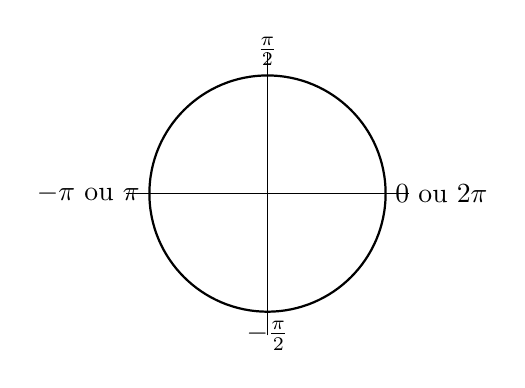
\begin{tikzpicture}[scale=1.5]
        % Axes
        \draw (0,-1.2) -- (0,1.2);
        \draw (-1.2,0) -- (1.2,0);
        
        % Cercle
        \draw[thick] (0,0) circle (1cm);
        
        % Labels des angles
        \node[right] at (1,0) {$0 \text{ ou } 2\pi$};
        \node[above] at (0,1) {$\frac{\pi}{2}$};
        \node[left] at (-1,0) {$-\pi \text{ ou } \pi$};
        \node[below] at (0,-1) {$-\frac{\pi}{2}$};
    \end{tikzpicture}
\end{center}


\noindent Soit $\alpha \in ]-\pi, \pi]$.

\begin{center}
    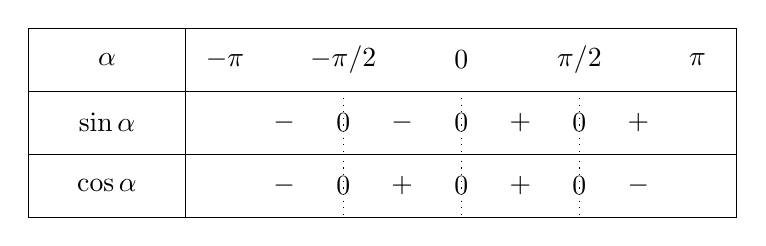
\begin{tikzpicture}
        \tkzTabInit[lgt=2, espcl=1.5]{$\alpha$ / .8, $\sin \alpha$ / .8, $\cos \alpha$ / .8}{$-\pi$, $-\pi/2$, $0$, $\pi/2$, $\pi$}
        \tkzTabLine{, -, z, -, z, +, z, +, }
        \tkzTabLine{, -, z, +, z, +, z, -, }
    \end{tikzpicture}
\end{center}
\vspace{1em}

\begin{center}
    \textcolor{monRouge}{\underline{\Large Application}}
\end{center}

\noindent \textbf{1)} Calculer $\cos x$, sachant que :
\[ \sin x = \dfrac{\sqrt{3}}{2} \quad \text{et} \quad \dfrac{\pi}{2} < x < \pi \]

\noindent \textbf{2)} Soit $x \in ]-\pi, 0[$ tel que : $\cos x = \dfrac{\sqrt{2}}{2}$. Déterminer la valeur de $\sin x$.

\noindent \textbf{3)} On donne $\tan x = \sqrt{3}$, $x \in ]0, \pi/2[$. Déterminer $\sin x$ et $\cos x$.

\begin{center}
    \textcolor{monRouge}{\underline{Correction}}
\end{center}

\noindent \textbf{1) Calculons $\cos x$} \\
On sait que $\cos^2 x + \sin^2 x = 1$ \\
$\cos^2 x = 1 - \sin^2 x$ \\
$\cos^2 x = 1 - \left( \dfrac{\sqrt{3}}{2} \right)^2$ \\
$\cos^2 x = 1 - \dfrac{3}{4}$ \\
$\cos^2 x = \dfrac{4-3}{4}$ \\
$\cos^2 x = \dfrac{1}{4}$ \\
$\cos x = \dfrac{1}{2} \quad \text{ou} \quad \cos x = -\dfrac{1}{2}$ \\
or $x \in \left] \pi/2, \pi \right[ \quad \text{donc} \quad \cos x < 0$

\vspace{1em}

\begin{center}
    \fbox{$\cos x = -\dfrac{1}{2}$}
\end{center}
\noindent \textbf{2) Déterminons la valeur de $\sin x$} \\
On sait que : $\cos^2 x + \sin^2 x = 1 \implies \sin^2 x = 1 - \cos^2 x$

\begin{align*}
    \sin^2 x &= 1 - \left( \frac{\sqrt{2}}{2} \right)^2 \\
    \sin^2 x &= 1 - \frac{2}{4} \\
    \sin^2 x &= \frac{2}{4} \\
    \sin x &= \frac{\sqrt{2}}{2} \quad \text{ou} \quad -\frac{\sqrt{2}}{2}
\end{align*}

\noindent Or $x \in ]-\pi, 0[$, donc $\sin x < 0$.

\begin{center}
    \fbox{$\sin x = -\dfrac{\sqrt{2}}{2}$}
\end{center}

\noindent \textbf{3) Déterminons $\sin x$ et $\cos x$} \\
On a : $1 + \tan^2 x = \dfrac{1}{\cos^2 x} \implies \cos^2 x = \dfrac{1}{1 + \tan^2 x}$

\begin{align*}
    \cos^2 x &= \dfrac{1}{1 + (\sqrt{3})^2} \text{} \\
    \cos^2 x &= \dfrac{1}{1 + 3} = \dfrac{1}{4} \text{} \\
    \cos x &= \frac{1}{2} \quad \text{ou} \quad \cos x = -\frac{1}{2} \text{}
\end{align*}

\noindent Or $x \in ]0, \pi/2[ \implies \cos x > 0$

\begin{center}
    \fbox{$\cos x = \dfrac{1}{2}$} \text{}
\end{center}

\noindent $\tan x = \dfrac{\sin x}{\cos x} \implies \sin x = \cos x \times \tan x$ \\
$\sin x = \frac{1}{2} \times \sqrt{3}$

\begin{center}
    \fbox{$\sin x = \dfrac{\sqrt{3}}{2}$} \text{}
\end{center}

\vspace{1.5em}

\subsection*{%
    \color{monRouge} \underline{d) Valeurs particulières de cosinus, sinus et tangente}%
}
\vspace{1em}

\noindent Le tableau suivant indique les valeurs remarquables des lignes trigonométriques à retenir.

\vspace{1em}

\begin{center}
    \begin{tabular}{|c|c|c|c|c|c|c|}
        \hline
        $\alpha$ & $0$ & $\frac{\pi}{6}$ & $\frac{\pi}{4}$ & $\frac{\pi}{3}$ & $\frac{\pi}{2}$ & $\pi$ \\
        \hline
        $\sin \alpha$ & $0$ & $\frac{1}{2}$ & $\frac{\sqrt{2}}{2}$ & $\frac{\sqrt{3}}{2}$ & $1$ & $0$ \\
        \hline
        $\cos \alpha$ & $1$ & $\frac{\sqrt{3}}{2}$ & $\frac{\sqrt{2}}{2}$ & $\frac{1}{2}$ & $0$ & $-1$ \\
        \hline
        $\tan \alpha$ & $0$ & $\frac{\sqrt{3}}{3}$ & $1$ & $\sqrt{3}$ & \fcolorbox{black}{gray!30}{\phantom{X}} & $0$ \\
        \hline
    \end{tabular}
\end{center}

\vspace{1.5em}

\begin{center}
    \textcolor{monRouge}{\underline{\Large Application}}
\end{center}

\noindent Calculer $\cos \left( \dfrac{97\pi}{4} \right)$ et $\sin \left( \dfrac{31\pi}{4} \right)$

\vspace{0.5em}

\begin{center}
    \textcolor{monRouge}{\underline{Correction}}
\end{center}

\noindent
\begin{minipage}[t]{0.45\textwidth}
    $\dfrac{97\pi}{4} = \dfrac{\pi + 4 \times 24\pi}{4}$ \\
    $\dfrac{97\pi}{4} = \dfrac{\pi}{4} + \dfrac{4 \times 24\pi}{4}$ \\
    $\dfrac{97\pi}{4} = \dfrac{\pi}{4} + 24\pi$ \\
    $\cos \left( \dfrac{97\pi}{4} \right) = \cos \left( \dfrac{\pi}{4} + 24\pi \right)$ \\
    \fbox{$\cos \left( \dfrac{97\pi}{4} \right) = \dfrac{\sqrt{2}}{2}$}
\end{minipage}
\hfill
\begin{minipage}[t]{0.45\textwidth}
    $\dfrac{31\pi}{3} = \dfrac{\pi + 3 \times 10\pi}{3}$ \\
    $\dfrac{31\pi}{3} = \dfrac{\pi}{3} + 10\pi$ \\
    $\sin \left( \dfrac{31\pi}{3} \right) = \sin \left( \dfrac{\pi}{3} + 10\pi \right)$ \\
    \fbox{$\sin \left( \dfrac{31\pi}{3} \right) = \dfrac{\sqrt{3}}{2}$}
\end{minipage}

\vspace{1.5em}

\subsection*{%
    \color{monRouge} \underline{2)Angles associés}%
}
\subsection*{%
    \color{monRouge} \underline{a) Angles opposés}%
}
\vspace{1em}

\begin{center}
    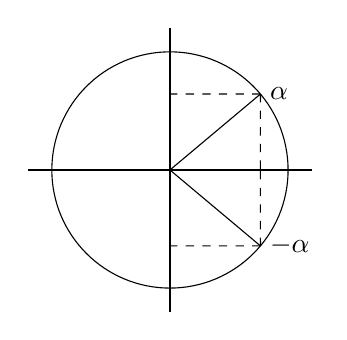
\begin{tikzpicture}[scale=1.5]
        % Axes
        \draw (0,-1.2) -- (0,1.2);
        \draw (-1.2,0) -- (1.2,0);
        % Cercle
        \draw (0,0) circle (1cm);
        % Points alpha et -alpha
        \coordinate (A) at (40:1);
        \coordinate (B) at (-40:1);
        \draw (0,0) -- (A) node[right] {$\alpha$};
        \draw (0,0) -- (B) node[right] {$-\alpha$};
        % Projections
        \draw[dashed] (A) -- ({cos(40)},0);
        \draw[dashed] (B) -- ({cos(40)},0);
        \draw[dashed] (A) -- (0,{sin(40)});
        \draw[dashed] (B) -- (0,{sin(-40)});
    \end{tikzpicture}
\end{center}

\textcolor{monRouge}{$\cos(-\alpha) = \cos(\alpha)$}

\textcolor{monRouge}{$\sin(-\alpha) = -\sin(\alpha)$}

\vspace{1.5em}

\subsection*{%
    \color{monRouge} \underline{b) Angles supplémentaire}%
}
\vspace{1em}

\textcolor{monRouge}{$ \alpha $} et \textcolor{monRouge}{$ \theta $} sont \textcolor{red}{supplémentaire} ssi \textcolor{red}{$ \alpha + \theta = \pi $} $(\theta = \pi - \alpha)$

\begin{center}
    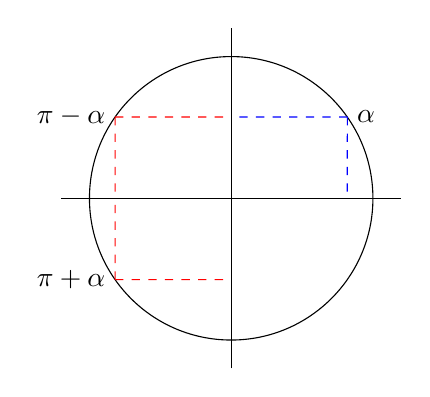
\begin{tikzpicture}[scale=1.8]
        % Axes
        \draw (0,-1.2) -- (0,1.2);
        \draw (-1.2,0) -- (1.2,0);
        % Cercle
        \draw (0,0) circle (1cm);
        
        % Points et angles
        \coordinate (alpha) at (35:1);
        \coordinate (pi_alpha) at (145:1);
        \coordinate (pi_plus_alpha) at (215:1);
        
        % Lignes de projection
        \draw[dashed, blue] (alpha) -- ({cos(35)},0);
        \draw[dashed, blue] (alpha) -- (0,{sin(35)});
        
        \draw[dashed, red] (pi_alpha) -- ({cos(145)},0);
        \draw[dashed, red] (pi_alpha) -- (0,{sin(145)});
        
        \draw[dashed, red] (pi_plus_alpha) -- ({cos(215)},0);
        \draw[dashed, red] (pi_plus_alpha) -- (0,{sin(215)});
        
        % Labels des points
        \node[right] at (alpha) {$\alpha$};
        \node[left] at (pi_alpha) {$\pi - \alpha$};
        \node[left] at (pi_plus_alpha) {$\pi + \alpha$};
    \end{tikzpicture}
\end{center}

\noindent \textbf{Pour tout réel $\alpha$, on a :} \\
\textcolor{red}{$\cos(\pi - \alpha) = -\cos \alpha$} \\
\textcolor{red}{$\sin(\pi - \alpha) = \sin \alpha$}

\noindent \textcolor{monRouge}{\underline{Remarque :}} \textbf{Pour tout réel $\alpha$, on a :} \\
\textcolor{red}{$\cos(\pi + \alpha) = -\cos \alpha$} \\
\textcolor{red}{$\sin(\pi + \alpha) = -\sin \alpha$}
\vspace{1.5em}

\subsection*{%
    \color{monRouge} \underline{b) Angles complémentaires}%
}
\vspace{1em}

Deux angles $\alpha$ et $\theta$ sont complémentaires ssi $\alpha + \theta = \dfrac{\pi}{2}$ \quad $\left( \theta = \dfrac{\pi}{2} - \alpha \right)$

\begin{center}
    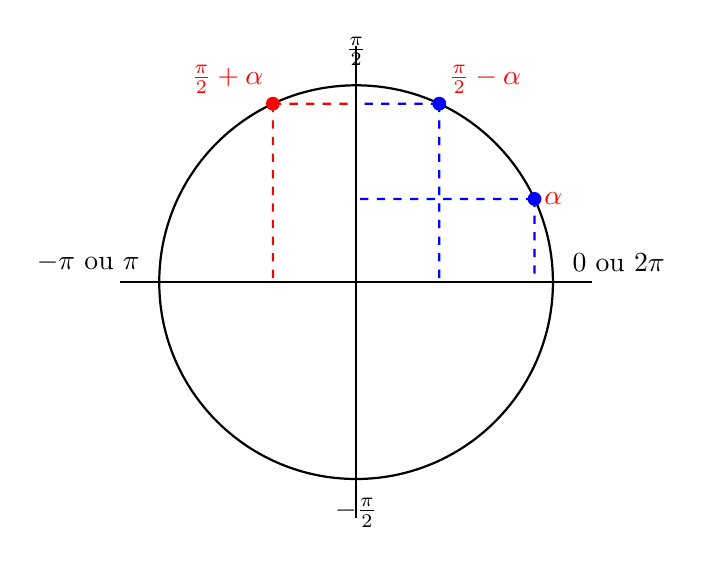
\begin{tikzpicture}[scale=2.5]
        % Axes principaux
        \draw[thick] (-1.2,0) -- (1.2,0);
        \draw[thick] (0,-1.2) -- (0,1.2);
        
        % Cercle trigonométrique
        \draw[thick] (0,0) circle (1cm);
        
        % Graduations des axes (comme sur ton dessin)
        \node[above] at (0,1.05) {$\frac{\pi}{2}$};
        \node[below] at (0,-1.05) {$-\frac{\pi}{2}$};
        \node[left] at (-1.05,0.1) {$-\pi$ ou $\pi$};
        \node[right] at (1.05,0.1) {$0$ ou $2\pi$};

        % Coordonnées des points (angles)
        \coordinate (alpha) at (25:1);
        \coordinate (pi_2_moins) at (65:1);
        \coordinate (pi_2_plus) at (115:1);
        
        % Pointillés bleus pour pi/2 - alpha et alpha
        \draw[dashed, blue, thick] (pi_2_moins) -- ({cos(65)},0);
        \draw[dashed, blue, thick] (pi_2_moins) -- (0,{sin(65)});
        \draw[dashed, blue, thick] (alpha) -- ({cos(25)},0);
        \draw[dashed, blue, thick] (alpha) -- (0,{sin(25)});
        
        % Pointillés rouges pour pi/2 + alpha
        \draw[dashed, red, thick] (pi_2_plus) -- ({cos(115)},0);
        \draw[dashed, red, thick] (pi_2_plus) -- (0,{sin(115)});

        % Labels des angles (en rouge comme sur le cahier)
        \node[right, red] at (alpha) {$\alpha$};
        \node[above right, red] at (pi_2_moins) {$\frac{\pi}{2} - \alpha$};
        \node[above left, red] at (pi_2_plus) {$\frac{\pi}{2} + \alpha$};
        
        % Petits points aux intersections
        \fill[blue] (alpha) circle (1pt);
        \fill[blue] (pi_2_moins) circle (1pt);
        \fill[red] (pi_2_plus) circle (1pt);

    \end{tikzpicture}
\end{center}

\noindent \textbf{Pour tout réel $\alpha$, on a :} \\
\textcolor{red}{ $\cos\left( \dfrac{\pi}{2} - \alpha \right) = \sin \alpha$} \quad;\quad
\textcolor{red}{ $\sin\left( \dfrac{\pi}{2} - \alpha \right) = \cos \alpha$}

\vspace{1em}

\noindent \textcolor{monRouge}{\underline{Remarque :}} \textbf{Pour tout réel $\alpha$, on a :} \\
\textcolor{red}{$\cos \left( \dfrac{\pi}{2} - \alpha \right) = -\sin \alpha$} \quad;\quad
\textcolor{red}{$\sin \left( \dfrac{\pi}{2} + \alpha \right) =  \cos \alpha$}

\subsection*{%
    \color{monRouge} \underline{C) Construction du trigonométrique}%
}
\vspace{1em}

\begin{figure}[H]
    \centering
    
\includegraphics[width=0.7\textwidth]{cercle1.png}
    \caption{Cercle Trigonométrique}
\end{figure}

\begin{center}
    \textcolor{monRouge}{\underline{\Large Application}}
\end{center}

\noindent Pour tout nombre réel $x$ appartenant à l'intervalle $\left] -\dfrac{\pi}{2}, \dfrac{\pi}{2} \right[$, on définit les nombres $A(x)$ et $B(x)$ par :

\vspace{1em}

\noindent $A(x) = \cos(-x) + \sin(-x) + \sin(\pi - x) - \cos(\pi - x)$ \\
$B(x) = \sin x + \sin\left( \dfrac{\pi}{2} - x \right) + \cos\left( \dfrac{\pi}{2} - x \right) - \cos\left( x - \dfrac{\pi}{2} \right)$

\vspace{1.5em}

\noindent \textbf{Mettre $A(x)$ et $B(x)$ sous la forme la plus simple possible}

\begin{center}
    \textcolor{monRouge}{\underline{Correction}}
\end{center}

\end{document}